\documentclass[aspectratio=169,11pt]{beamer}
% =====================================================================
%  pds-beamer.tex — Estilo común de las transparencias.
%
%  Uso (desde teoría/Tx/transparencias/):
%     \documentclass[aspectratio=169,11pt]{beamer}
%     % =====================================================================
%  pds-beamer.tex — Estilo común de las transparencias.
%
%  Uso (desde teoría/Tx/transparencias/):
%     \documentclass[aspectratio=169,11pt]{beamer}
%     % =====================================================================
%  pds-beamer.tex — Estilo común de las transparencias.
%
%  Uso (desde teoría/Tx/transparencias/):
%     \documentclass[aspectratio=169,11pt]{beamer}
%     \input{../../comun/pds-beamer}
%     \title{...}  \subtitle{Tema x · ...}
%     \begin{document}
%       \portada
%       ...
%     \end{document}
%  Compilar con:  latexmk -xelatex  (o «make» desde teoría/)
% =====================================================================

\usetheme{Boadilla}
\usecolortheme{orchid}
\usefonttheme{professionalfonts}
\setbeamercovered{transparent}
\setbeamersize{text margin left=0.8cm, text margin right=0.8cm}
\setbeamertemplate{navigation symbols}{}
\setbeamertemplate{itemize item}[square]
\setbeamertemplate{itemize subitem}[circle]
\setbeamertemplate{itemize subsubitem}[triangle]
\setbeamertemplate{enumerate item}[square]
\setbeamertemplate{enumerate subitem}[circle]
\setbeamertemplate{caption}{\raggedright\insertcaption\par}

\input{../../comun/pds-comun.tex}

% Tipografía: Fira Sans + Fira Math (legibles en proyector)
\usepackage{fontspec}
\usepackage{unicode-math}
% Se cargan por nombre de fichero para que funcionen con cualquier
% instalación de TeX Live (o MiKTeX) sin instalar fuentes en el sistema.
\setmainfont{FiraSans}[Extension=.otf, UprightFont=*-Regular, BoldFont=*-SemiBold,
  ItalicFont=*-Italic, BoldItalicFont=*-SemiBoldItalic]
\setsansfont{FiraSans}[Extension=.otf, UprightFont=*-Regular, BoldFont=*-SemiBold,
  ItalicFont=*-Italic, BoldItalicFont=*-SemiBoldItalic]
\setmonofont{FiraMono}[Extension=.otf, UprightFont=*-Regular, BoldFont=*-Medium, AutoFakeSlant=0.15, Scale=0.92]
\setmathfont{FiraMath-Regular.otf}
\setmathfont{latinmodern-math.otf}[range={"229B,"22EE,"22F1}]

% Colores del tema ajustados a la paleta común (más contraste)
\setbeamercolor{structure}{fg=pdsazul}
\setbeamercolor{alerted text}{fg=pdsrojo}
\setbeamercolor{example text}{fg=pdsverde}
\setbeamercolor{block title}{bg=pdsazul, fg=white}
\setbeamercolor{block body}{bg=pdsfondo}
\setbeamercolor{block title alerted}{bg=pdsrojo, fg=white}
\setbeamercolor{block body alerted}{bg=pdsrojo!6}
\setbeamercolor{block title example}{bg=pdsverde, fg=white}
\setbeamercolor{block body example}{bg=pdsverde!6}
\setbeamercolor{frametitle}{fg=pdsazul, bg=white}
\setbeamerfont{frametitle}{size=\large, series=\bfseries}
\setbeamerfont{block title}{size=\normalsize, series=\bfseries}
\setbeamertemplate{blocks}[rounded][shadow=false]

% Logo en la esquina superior derecha de cada transparencia
\pgfdeclareimage[height=0.8cm]{logo}{../../comun/ucm.png}
\addtobeamertemplate{frametitle}{}{%
  \begin{tikzpicture}[remember picture, overlay]
    \node[anchor=north east, inner sep=0pt] at ([xshift=-0.25cm, yshift=-0.2cm]current page.north east) {\pgfuseimage{logo}};
  \end{tikzpicture}}

% Datos de portada
\author[\autorescorto]{\autores}
\institute[UCM]{\footnotesize\departamento\\\universidad}
\date[\curso]{\footnotesize\grado\\\curso}

\newcommand{\portada}{%
  \begin{frame}[plain]
    \begin{center}
      
\includegraphics[height=1.9cm]{../../comun/ucm.png}
    \end{center}
    \vspace{-0.4cm}
    \titlepage
  \end{frame}}

% Índice al empezar cada sección
\AtBeginSection[]{%
  \begin{frame}{Contenido}
    \tableofcontents[currentsection, hideothersubsections]
  \end{frame}}

\renewcommand{\pdscodesize}{\scriptsize}

% Utilidades
% \herramienta{T1-convolucion-continua}: enlace a la página publicada de
% herramientas/html (se abre en el navegador, sin instalar nada).
% \herramientaservidor{server/....py}: app que necesita Python (bokeh serve).
\newcommand{\urlherramientas}{https://ucm-237.github.io/PdS/}
\newcommand{\herramienta}[1]{%
  \par\vfill\hfill{\scriptsize\color{pdsgris}\faIcon\ \href{\urlherramientas#1.html}{Herramienta interactiva: \texttt{#1}}}}
\newcommand{\herramientaservidor}[1]{%
  \par\vfill\hfill{\scriptsize\color{pdsgris}\faIcon\ Herramienta interactiva (con Python): \texttt{herramientas/#1}}}
\newcommand{\faIcon}{\textbf{▶}}
\newcommand{\gris}[1]{{\color{pdsgris}#1}}
\newcommand{\nota}[1]{\par\vspace{2pt}{\footnotesize\color{pdsgris}\textit{#1}}\par}
% Nota sobre una errata de versiones anteriores (solo con \ERRATAS)
\newcommand{\errata}[1]{\iferratas\nota{Errata de versiones anteriores: #1}\fi}
\newcommand{\apuntes}[1]{\nota{Más detalle en los apuntes, #1.}}

% Bloques con nombre en castellano
\newenvironment{definicion}[1][Definición]{\begin{block}{#1}}{\end{block}}
\newenvironment{importante}[1][Importante]{\begin{alertblock}{#1}}{\end{alertblock}}
\newenvironment{ejemplo}[1][Ejemplo]{\begin{exampleblock}{#1}}{\end{exampleblock}}

%     \title{...}  \subtitle{Tema x · ...}
%     \begin{document}
%       \portada
%       ...
%     \end{document}
%  Compilar con:  latexmk -xelatex  (o «make» desde teoría/)
% =====================================================================

\usetheme{Boadilla}
\usecolortheme{orchid}
\usefonttheme{professionalfonts}
\setbeamercovered{transparent}
\setbeamersize{text margin left=0.8cm, text margin right=0.8cm}
\setbeamertemplate{navigation symbols}{}
\setbeamertemplate{itemize item}[square]
\setbeamertemplate{itemize subitem}[circle]
\setbeamertemplate{itemize subsubitem}[triangle]
\setbeamertemplate{enumerate item}[square]
\setbeamertemplate{enumerate subitem}[circle]
\setbeamertemplate{caption}{\raggedright\insertcaption\par}

% =====================================================================
%  pds-comun.tex — Paquetes, colores y estilos de código comunes a
%  transparencias, apuntes y hojas de ejercicios. Compilar con XeLaTeX.
%  No cargar directamente: lo cargan pds-beamer.tex y pds-apuntes.tex.
% =====================================================================

\usepackage{polyglossia}
\setmainlanguage{spanish}
\usepackage{mathtools}
\usepackage{graphicx}
\usepackage{booktabs}
\usepackage{multirow}
\usepackage{array}
\usepackage{xcolor}
\usepackage{tikz}
\usetikzlibrary{positioning,arrows.meta,calc,shapes.geometric,decorations.pathreplacing}
\usepackage{listings}
\usepackage{siunitx}
\sisetup{output-decimal-marker={,}, group-separator={\,}, per-mode=symbol}

% Notas de erratas de versiones anteriores: no se imprimen salvo que se
% defina \ERRATAS antes de cargar el estilo (make ERRATAS=1)
\newif\iferratas
\ifdefined\ERRATAS \erratastrue \fi

% Ruta común (logo y figuras compartidas)
\providecommand{\rutacomun}{../../comun/}
\input{\rutacomun datos.tex}

% ---------------------------------------------------------------------
%  Paleta (la misma que usan las figuras generadas con Python,
%  ver comun/pds_estilo.py)
% ---------------------------------------------------------------------
\definecolor{pdsazul}{HTML}{2B3A8C}
\definecolor{pdsrojo}{HTML}{C0392B}
\definecolor{pdsverde}{HTML}{1E7B4F}
\definecolor{pdsnaranja}{HTML}{D9822B}
\definecolor{pdsgris}{HTML}{5A5A66}
\definecolor{pdsfondo}{HTML}{F3F4FA}
\definecolor{pdscodigo}{HTML}{F7F7F2}

% ---------------------------------------------------------------------
%  Diagramas de bloques (TikZ)
% ---------------------------------------------------------------------
\tikzset{
  bloque/.style={rectangle, rounded corners=2pt, draw=pdsazul!80, fill=pdsfondo,
                 very thick, minimum height=8mm, minimum width=14mm, align=center},
  sumador/.style={circle, draw=pdsazul!80, fill=pdsfondo, thick, inner sep=1.5pt},
  flecha/.style={-{Stealth[length=2.2mm]}, thick, pdsgris},
}

% ---------------------------------------------------------------------
%  Código: Python y Matlab en paralelo
% ---------------------------------------------------------------------
\newcommand{\pdscodesize}{\footnotesize}
\lstdefinestyle{pds}{
  basicstyle=\ttfamily\pdscodesize,
  keywordstyle=\color{pdsazul}\bfseries,
  commentstyle=\color{pdsverde}\itshape,
  stringstyle=\color{pdsrojo},
  numbers=none,
  backgroundcolor=\color{pdscodigo},
  frame=single, rulecolor=\color{pdsgris!40}, framerule=0.4pt,
  xleftmargin=2pt, xrightmargin=2pt, aboveskip=2pt, belowskip=2pt,
  columns=fullflexible, keepspaces=true,
  showstringspaces=false, breaklines=true, tabsize=4,
  upquote=true,
  % Con XeLaTeX, listings desordena los caracteres no ASCII junto a
  % dígitos («2π» sale «π2»): se sustituyen por su versión matemática.
  literate={π}{{$\pi$}}1 {δ}{{$\delta$}}1 {ω}{{$\omega$}}1 {Ω}{{$\Omega$}}1
           {≈}{{$\approx$}}1 {µ}{{$\mu$}}1 {·}{{$\cdot$}}1 {α}{{$\alpha$}}1
           {á}{{á}}1 {é}{{é}}1 {í}{{í}}1 {ó}{{ó}}1 {ú}{{ú}}1 {ñ}{{ñ}}1 {¿}{{¿}}1,
}
\lstdefinestyle{python}{style=pds, language=Python,
  morekeywords={as,True,False,None}}
\lstdefinestyle{matlab}{style=pds, language=Matlab,
  morekeywords={function,end,true,false}}

% \codigo{<ruta sin extensión>} muestra el mismo ejemplo en Python
% y en Matlab, uno al lado del otro. Los ficheros viven en
% ../codigo/python/<nombre>.py y ../codigo/matlab/<nombre>.m y se
% ejecutan en las pruebas (make prueba-codigo).
\newcommand{\rutacodigo}{../codigo/}
\newcommand{\codigoetiqueta}[1]{{\sffamily\scriptsize\bfseries\color{pdsgris}#1}}
\newcommand{\codigo}[2][]{%
  \par\noindent
  \begin{minipage}[t]{0.495\linewidth}
    \codigoetiqueta{Python}\par\vspace{1pt}
    \lstinputlisting[style=python,#1]{\rutacodigo python/#2.py}
  \end{minipage}\hfill
  \begin{minipage}[t]{0.495\linewidth}
    \codigoetiqueta{Matlab}\par\vspace{1pt}
    \lstinputlisting[style=matlab,#1]{\rutacodigo matlab/#2.m}
  \end{minipage}\par}

\input{\rutacomun notacion.tex}


% Tipografía: Fira Sans + Fira Math (legibles en proyector)
\usepackage{fontspec}
\usepackage{unicode-math}
% Se cargan por nombre de fichero para que funcionen con cualquier
% instalación de TeX Live (o MiKTeX) sin instalar fuentes en el sistema.
\setmainfont{FiraSans}[Extension=.otf, UprightFont=*-Regular, BoldFont=*-SemiBold,
  ItalicFont=*-Italic, BoldItalicFont=*-SemiBoldItalic]
\setsansfont{FiraSans}[Extension=.otf, UprightFont=*-Regular, BoldFont=*-SemiBold,
  ItalicFont=*-Italic, BoldItalicFont=*-SemiBoldItalic]
\setmonofont{FiraMono}[Extension=.otf, UprightFont=*-Regular, BoldFont=*-Medium, AutoFakeSlant=0.15, Scale=0.92]
\setmathfont{FiraMath-Regular.otf}
\setmathfont{latinmodern-math.otf}[range={"229B,"22EE,"22F1}]

% Colores del tema ajustados a la paleta común (más contraste)
\setbeamercolor{structure}{fg=pdsazul}
\setbeamercolor{alerted text}{fg=pdsrojo}
\setbeamercolor{example text}{fg=pdsverde}
\setbeamercolor{block title}{bg=pdsazul, fg=white}
\setbeamercolor{block body}{bg=pdsfondo}
\setbeamercolor{block title alerted}{bg=pdsrojo, fg=white}
\setbeamercolor{block body alerted}{bg=pdsrojo!6}
\setbeamercolor{block title example}{bg=pdsverde, fg=white}
\setbeamercolor{block body example}{bg=pdsverde!6}
\setbeamercolor{frametitle}{fg=pdsazul, bg=white}
\setbeamerfont{frametitle}{size=\large, series=\bfseries}
\setbeamerfont{block title}{size=\normalsize, series=\bfseries}
\setbeamertemplate{blocks}[rounded][shadow=false]

% Logo en la esquina superior derecha de cada transparencia
\pgfdeclareimage[height=0.8cm]{logo}{../../comun/ucm.png}
\addtobeamertemplate{frametitle}{}{%
  \begin{tikzpicture}[remember picture, overlay]
    \node[anchor=north east, inner sep=0pt] at ([xshift=-0.25cm, yshift=-0.2cm]current page.north east) {\pgfuseimage{logo}};
  \end{tikzpicture}}

% Datos de portada
\author[\autorescorto]{\autores}
\institute[UCM]{\footnotesize\departamento\\\universidad}
\date[\curso]{\footnotesize\grado\\\curso}

\newcommand{\portada}{%
  \begin{frame}[plain]
    \begin{center}
      
\includegraphics[height=1.9cm]{../../comun/ucm.png}
    \end{center}
    \vspace{-0.4cm}
    \titlepage
  \end{frame}}

% Índice al empezar cada sección
\AtBeginSection[]{%
  \begin{frame}{Contenido}
    \tableofcontents[currentsection, hideothersubsections]
  \end{frame}}

\renewcommand{\pdscodesize}{\scriptsize}

% Utilidades
% \herramienta{T1-convolucion-continua}: enlace a la página publicada de
% herramientas/html (se abre en el navegador, sin instalar nada).
% \herramientaservidor{server/....py}: app que necesita Python (bokeh serve).
\newcommand{\urlherramientas}{https://ucm-237.github.io/PdS/}
\newcommand{\herramienta}[1]{%
  \par\vfill\hfill{\scriptsize\color{pdsgris}\faIcon\ \href{\urlherramientas#1.html}{Herramienta interactiva: \texttt{#1}}}}
\newcommand{\herramientaservidor}[1]{%
  \par\vfill\hfill{\scriptsize\color{pdsgris}\faIcon\ Herramienta interactiva (con Python): \texttt{herramientas/#1}}}
\newcommand{\faIcon}{\textbf{▶}}
\newcommand{\gris}[1]{{\color{pdsgris}#1}}
\newcommand{\nota}[1]{\par\vspace{2pt}{\footnotesize\color{pdsgris}\textit{#1}}\par}
% Nota sobre una errata de versiones anteriores (solo con \ERRATAS)
\newcommand{\errata}[1]{\iferratas\nota{Errata de versiones anteriores: #1}\fi}
\newcommand{\apuntes}[1]{\nota{Más detalle en los apuntes, #1.}}

% Bloques con nombre en castellano
\newenvironment{definicion}[1][Definición]{\begin{block}{#1}}{\end{block}}
\newenvironment{importante}[1][Importante]{\begin{alertblock}{#1}}{\end{alertblock}}
\newenvironment{ejemplo}[1][Ejemplo]{\begin{exampleblock}{#1}}{\end{exampleblock}}

%     \title{...}  \subtitle{Tema x · ...}
%     \begin{document}
%       \portada
%       ...
%     \end{document}
%  Compilar con:  latexmk -xelatex  (o «make» desde teoría/)
% =====================================================================

\usetheme{Boadilla}
\usecolortheme{orchid}
\usefonttheme{professionalfonts}
\setbeamercovered{transparent}
\setbeamersize{text margin left=0.8cm, text margin right=0.8cm}
\setbeamertemplate{navigation symbols}{}
\setbeamertemplate{itemize item}[square]
\setbeamertemplate{itemize subitem}[circle]
\setbeamertemplate{itemize subsubitem}[triangle]
\setbeamertemplate{enumerate item}[square]
\setbeamertemplate{enumerate subitem}[circle]
\setbeamertemplate{caption}{\raggedright\insertcaption\par}

% =====================================================================
%  pds-comun.tex — Paquetes, colores y estilos de código comunes a
%  transparencias, apuntes y hojas de ejercicios. Compilar con XeLaTeX.
%  No cargar directamente: lo cargan pds-beamer.tex y pds-apuntes.tex.
% =====================================================================

\usepackage{polyglossia}
\setmainlanguage{spanish}
\usepackage{mathtools}
\usepackage{graphicx}
\usepackage{booktabs}
\usepackage{multirow}
\usepackage{array}
\usepackage{xcolor}
\usepackage{tikz}
\usetikzlibrary{positioning,arrows.meta,calc,shapes.geometric,decorations.pathreplacing}
\usepackage{listings}
\usepackage{siunitx}
\sisetup{output-decimal-marker={,}, group-separator={\,}, per-mode=symbol}

% Notas de erratas de versiones anteriores: no se imprimen salvo que se
% defina \ERRATAS antes de cargar el estilo (make ERRATAS=1)
\newif\iferratas
\ifdefined\ERRATAS \erratastrue \fi

% Ruta común (logo y figuras compartidas)
\providecommand{\rutacomun}{../../comun/}
\input{\rutacomun datos.tex}

% ---------------------------------------------------------------------
%  Paleta (la misma que usan las figuras generadas con Python,
%  ver comun/pds_estilo.py)
% ---------------------------------------------------------------------
\definecolor{pdsazul}{HTML}{2B3A8C}
\definecolor{pdsrojo}{HTML}{C0392B}
\definecolor{pdsverde}{HTML}{1E7B4F}
\definecolor{pdsnaranja}{HTML}{D9822B}
\definecolor{pdsgris}{HTML}{5A5A66}
\definecolor{pdsfondo}{HTML}{F3F4FA}
\definecolor{pdscodigo}{HTML}{F7F7F2}

% ---------------------------------------------------------------------
%  Diagramas de bloques (TikZ)
% ---------------------------------------------------------------------
\tikzset{
  bloque/.style={rectangle, rounded corners=2pt, draw=pdsazul!80, fill=pdsfondo,
                 very thick, minimum height=8mm, minimum width=14mm, align=center},
  sumador/.style={circle, draw=pdsazul!80, fill=pdsfondo, thick, inner sep=1.5pt},
  flecha/.style={-{Stealth[length=2.2mm]}, thick, pdsgris},
}

% ---------------------------------------------------------------------
%  Código: Python y Matlab en paralelo
% ---------------------------------------------------------------------
\newcommand{\pdscodesize}{\footnotesize}
\lstdefinestyle{pds}{
  basicstyle=\ttfamily\pdscodesize,
  keywordstyle=\color{pdsazul}\bfseries,
  commentstyle=\color{pdsverde}\itshape,
  stringstyle=\color{pdsrojo},
  numbers=none,
  backgroundcolor=\color{pdscodigo},
  frame=single, rulecolor=\color{pdsgris!40}, framerule=0.4pt,
  xleftmargin=2pt, xrightmargin=2pt, aboveskip=2pt, belowskip=2pt,
  columns=fullflexible, keepspaces=true,
  showstringspaces=false, breaklines=true, tabsize=4,
  upquote=true,
  % Con XeLaTeX, listings desordena los caracteres no ASCII junto a
  % dígitos («2π» sale «π2»): se sustituyen por su versión matemática.
  literate={π}{{$\pi$}}1 {δ}{{$\delta$}}1 {ω}{{$\omega$}}1 {Ω}{{$\Omega$}}1
           {≈}{{$\approx$}}1 {µ}{{$\mu$}}1 {·}{{$\cdot$}}1 {α}{{$\alpha$}}1
           {á}{{á}}1 {é}{{é}}1 {í}{{í}}1 {ó}{{ó}}1 {ú}{{ú}}1 {ñ}{{ñ}}1 {¿}{{¿}}1,
}
\lstdefinestyle{python}{style=pds, language=Python,
  morekeywords={as,True,False,None}}
\lstdefinestyle{matlab}{style=pds, language=Matlab,
  morekeywords={function,end,true,false}}

% \codigo{<ruta sin extensión>} muestra el mismo ejemplo en Python
% y en Matlab, uno al lado del otro. Los ficheros viven en
% ../codigo/python/<nombre>.py y ../codigo/matlab/<nombre>.m y se
% ejecutan en las pruebas (make prueba-codigo).
\newcommand{\rutacodigo}{../codigo/}
\newcommand{\codigoetiqueta}[1]{{\sffamily\scriptsize\bfseries\color{pdsgris}#1}}
\newcommand{\codigo}[2][]{%
  \par\noindent
  \begin{minipage}[t]{0.495\linewidth}
    \codigoetiqueta{Python}\par\vspace{1pt}
    \lstinputlisting[style=python,#1]{\rutacodigo python/#2.py}
  \end{minipage}\hfill
  \begin{minipage}[t]{0.495\linewidth}
    \codigoetiqueta{Matlab}\par\vspace{1pt}
    \lstinputlisting[style=matlab,#1]{\rutacodigo matlab/#2.m}
  \end{minipage}\par}

\input{\rutacomun notacion.tex}


% Tipografía: Fira Sans + Fira Math (legibles en proyector)
\usepackage{fontspec}
\usepackage{unicode-math}
% Se cargan por nombre de fichero para que funcionen con cualquier
% instalación de TeX Live (o MiKTeX) sin instalar fuentes en el sistema.
\setmainfont{FiraSans}[Extension=.otf, UprightFont=*-Regular, BoldFont=*-SemiBold,
  ItalicFont=*-Italic, BoldItalicFont=*-SemiBoldItalic]
\setsansfont{FiraSans}[Extension=.otf, UprightFont=*-Regular, BoldFont=*-SemiBold,
  ItalicFont=*-Italic, BoldItalicFont=*-SemiBoldItalic]
\setmonofont{FiraMono}[Extension=.otf, UprightFont=*-Regular, BoldFont=*-Medium, AutoFakeSlant=0.15, Scale=0.92]
\setmathfont{FiraMath-Regular.otf}
\setmathfont{latinmodern-math.otf}[range={"229B,"22EE,"22F1}]

% Colores del tema ajustados a la paleta común (más contraste)
\setbeamercolor{structure}{fg=pdsazul}
\setbeamercolor{alerted text}{fg=pdsrojo}
\setbeamercolor{example text}{fg=pdsverde}
\setbeamercolor{block title}{bg=pdsazul, fg=white}
\setbeamercolor{block body}{bg=pdsfondo}
\setbeamercolor{block title alerted}{bg=pdsrojo, fg=white}
\setbeamercolor{block body alerted}{bg=pdsrojo!6}
\setbeamercolor{block title example}{bg=pdsverde, fg=white}
\setbeamercolor{block body example}{bg=pdsverde!6}
\setbeamercolor{frametitle}{fg=pdsazul, bg=white}
\setbeamerfont{frametitle}{size=\large, series=\bfseries}
\setbeamerfont{block title}{size=\normalsize, series=\bfseries}
\setbeamertemplate{blocks}[rounded][shadow=false]

% Logo en la esquina superior derecha de cada transparencia
\pgfdeclareimage[height=0.8cm]{logo}{../../comun/ucm.png}
\addtobeamertemplate{frametitle}{}{%
  \begin{tikzpicture}[remember picture, overlay]
    \node[anchor=north east, inner sep=0pt] at ([xshift=-0.25cm, yshift=-0.2cm]current page.north east) {\pgfuseimage{logo}};
  \end{tikzpicture}}

% Datos de portada
\author[\autorescorto]{\autores}
\institute[UCM]{\footnotesize\departamento\\\universidad}
\date[\curso]{\footnotesize\grado\\\curso}

\newcommand{\portada}{%
  \begin{frame}[plain]
    \begin{center}
      
\includegraphics[height=1.9cm]{../../comun/ucm.png}
    \end{center}
    \vspace{-0.4cm}
    \titlepage
  \end{frame}}

% Índice al empezar cada sección
\AtBeginSection[]{%
  \begin{frame}{Contenido}
    \tableofcontents[currentsection, hideothersubsections]
  \end{frame}}

\renewcommand{\pdscodesize}{\scriptsize}

% Utilidades
% \herramienta{T1-convolucion-continua}: enlace a la página publicada de
% herramientas/html (se abre en el navegador, sin instalar nada).
% \herramientaservidor{server/....py}: app que necesita Python (bokeh serve).
\newcommand{\urlherramientas}{https://ucm-237.github.io/PdS/}
\newcommand{\herramienta}[1]{%
  \par\vfill\hfill{\scriptsize\color{pdsgris}\faIcon\ \href{\urlherramientas#1.html}{Herramienta interactiva: \texttt{#1}}}}
\newcommand{\herramientaservidor}[1]{%
  \par\vfill\hfill{\scriptsize\color{pdsgris}\faIcon\ Herramienta interactiva (con Python): \texttt{herramientas/#1}}}
\newcommand{\faIcon}{\textbf{▶}}
\newcommand{\gris}[1]{{\color{pdsgris}#1}}
\newcommand{\nota}[1]{\par\vspace{2pt}{\footnotesize\color{pdsgris}\textit{#1}}\par}
% Nota sobre una errata de versiones anteriores (solo con \ERRATAS)
\newcommand{\errata}[1]{\iferratas\nota{Errata de versiones anteriores: #1}\fi}
\newcommand{\apuntes}[1]{\nota{Más detalle en los apuntes, #1.}}

% Bloques con nombre en castellano
\newenvironment{definicion}[1][Definición]{\begin{block}{#1}}{\end{block}}
\newenvironment{importante}[1][Importante]{\begin{alertblock}{#1}}{\end{alertblock}}
\newenvironment{ejemplo}[1][Ejemplo]{\begin{exampleblock}{#1}}{\end{exampleblock}}

\graphicspath{{../figuras/}}

\title[T4 · Filtros continuos]{Filtros}
\subtitle{Tema 4 · Parte 2: filtros continuos}

\begin{document}
\portada

% =====================================================================
\section{Planteamiento}

\begin{frame}{Diseño por aproximación del módulo}
  \small
  \begin{itemize}
    \item Buscamos $H(s)$ racional, causal y estable cuyo módulo aproxime al paso bajo ideal. Se diseña $\abs{H(j\omega)}^2$, que es una función par de $\omega$:
    \[
      \abs{H(j\omega)}^2=\frac{1}{1+P(\omega^2)},
    \]
    con $P$ pequeño en la banda de paso y grande en la de supresión.
    \item Elegir $P$ es elegir la familia (Butterworth, Chebyshev, elíptico). De $H(s)H(-s)$ se toman los polos del semiplano izquierdo.
    \item Solo se diseña el \alert{paso bajo prototipo}; los demás tipos se obtienen con una transformación de frecuencias (sección 3).
  \end{itemize}
  \begin{importante}[Datos del diseño]
    $\omega_p$, $\omega_s$ (rad/s), $\alpha_p$, $\alpha_s$ (dB) $\ \to\ $ $E=10^{\alpha_p/20}$, $A=10^{\alpha_s/20}$, $\varepsilon=\sqrt{E^2-1}$, $k=\dfrac{\omega_p}{\omega_s}$, $k_1=\dfrac{\varepsilon}{\sqrt{A^2-1}}$.
  \end{importante}
\end{frame}

% =====================================================================
\section{Butterworth}

\begin{frame}{Filtro de Butterworth}
  \begin{columns}[c]
    \begin{column}{0.48\textwidth}
      \[
        \abs{H(j\omega)}^2=\frac{1}{1+(\omega/\omega_c)^{2N}}
      \]
      \begin{itemize}\small
        \item \alert{Máximamente plano}: las $2N-1$ primeras derivadas son nulas en $\omega=0$.
        \item Monótono; $-3$\,dB en $\omega_c$ para cualquier $N$; cae $20N$\,dB/década.
        \item Polos sobre una circunferencia de radio $\omega_c$, separados $\pi/N$:
        \[
          p_k=\omega_c\,\e^{j\pi\frac{2k+N-1}{2N}},\ k=1,\dots,N.
        \]
      \end{itemize}
    \end{column}
    \begin{column}{0.5\textwidth}
      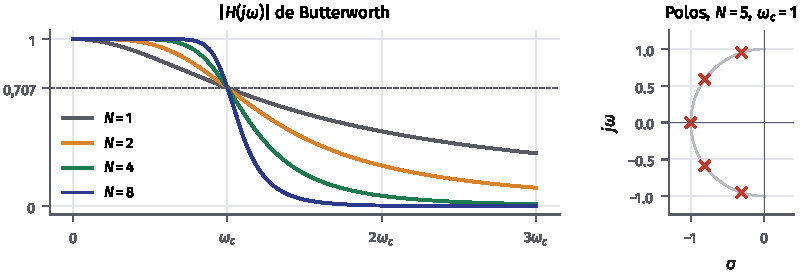
\includegraphics[width=\linewidth]{butterworth_orden}
    \end{column}
  \end{columns}
\end{frame}

\begin{frame}{Butterworth: orden y frecuencia de corte}
  Imponemos la plantilla en los bordes:
  \[
    \frac{1}{1+(\omega_p/\omega_c)^{2N}}\ge\frac1{E^2},\qquad
    \frac{1}{1+(\omega_s/\omega_c)^{2N}}\le\frac1{A^2}
    \ \Rightarrow\
    \Big(\frac{\omega_s}{\omega_p}\Big)^{2N}\ge\frac{A^2-1}{E^2-1}
  \]
  \begin{importante}[Orden mínimo]
    \[
      N\ge\frac{\log_{10}\dfrac{A^2-1}{E^2-1}}{2\log_{10}\dfrac{\omega_s}{\omega_p}}=\frac{\log(1/k_1)}{\log(1/k)},
      \qquad
      \frac{\omega_p}{(E^2-1)^{1/2N}}\le\omega_c\le\frac{\omega_s}{(A^2-1)^{1/2N}}
    \]
  \end{importante}
  \begin{itemize}\small
    \item $N$ se redondea hacia arriba; queda margen y $\omega_c$ puede elegirse en un intervalo.
    \item El extremo izquierdo cumple la banda de paso exactamente; el derecho, la de supresión. \texttt{buttord} devuelve el izquierdo.
  \end{itemize}
\end{frame}

\begin{frame}{Ejemplo: Butterworth}
  \begin{ejemplo}[Enunciado]
    Paso bajo de orden mínimo con atenuación máxima de 1\,dB hasta 1\,kHz y mínima de 40\,dB desde 5\,kHz.
  \end{ejemplo}
  \begin{align*}
    &\omega_p=2\pi\cdot1000,\quad \omega_s=2\pi\cdot5000,\quad E=10^{1/20}=1{,}122,\quad A=10^{40/20}=100\\
    &N\ge\frac{\log_{10}(9999/0{,}2589)}{2\log_{10}5}=3{,}28\ \to\ N=4\\
    &\omega_c\in\Big[\frac{\omega_p}{0{,}2589^{1/8}},\ \frac{\omega_s}{9999^{1/8}}\Big]=[7439,\ 9935]\ \text{rad/s}
  \end{align*}
  \nota{En hercios, $f_c$ entre 1184 y 1581\,Hz. Con $\omega_c=7439$ la atenuación en 1\,kHz es exactamente 1\,dB y en 5\,kHz supera los 40\,dB.}
\end{frame}

\begin{frame}{En código: Butterworth continuo}
  \codigo{butter_continuo}
  \nota{\texttt{freqs} evalúa $H(j\omega)$ de un filtro continuo; \texttt{freqz}, $H(\e^{j\Omega})$ de uno discreto.}
\end{frame}

% =====================================================================
\section{Chebyshev y elíptico}

\begin{frame}{Polinomios de Chebyshev}
  \begin{columns}[c]
    \begin{column}{0.55\textwidth}
      \[
        T_N(x)=\begin{cases}\cos(N\arccos x) & \abs x\le1\\ \cosh(N\,\mathrm{arccosh}\,x) & \abs x>1\end{cases}
      \]
      \begin{itemize}\small
        \item Recurrencia: $T_0=1$, $T_1=x$, $T_{N+1}=2xT_N-T_{N-1}$. Por ejemplo, $T_2=2x^2-1$, $T_3=4x^3-3x$.
        \item En $[-1,1]$ oscila entre $-1$ y $1$ (equirrizado); fuera crece como $2^{N-1}x^N$, mucho más deprisa que $x^N$.
        \item Por eso un Chebyshev cae más deprisa que un Butterworth del mismo orden.
      \end{itemize}
    \end{column}
    \begin{column}{0.43\textwidth}
      \begin{importante}[Chebyshev tipo I]
        \[
          \abs{H(j\omega)}^2=\frac{1}{1+\varepsilon^2T_N^2(\omega/\omega_p)}
        \]
        \small Rizado entre $1$ y $1/E$ en la banda de paso; monótono en la de supresión; polos sobre una elipse.
      \end{importante}
    \end{column}
  \end{columns}
\end{frame}

\begin{frame}{Chebyshev tipo I y tipo II}
  \small
  \begin{itemize}
    \item \alert{Tipo I}: en $\omega_s$, $1+\varepsilon^2\cosh^2(N\,\mathrm{arccosh}(\omega_s/\omega_p))\ge A^2$:
    \[
      N\ge\frac{\mathrm{arccosh}(1/k_1)}{\mathrm{arccosh}(1/k)}=\frac{\mathrm{arccosh}\big(\sqrt{A^2-1}/\varepsilon\big)}{\mathrm{arccosh}(\omega_s/\omega_p)}.
    \]
    \item \alert{Tipo II} (inverso): plano en la banda de paso, rizado en la de supresión y ceros sobre el eje $j\omega$:
    \[
      \abs{H(j\omega)}^2=\frac{\varepsilon_2^2\,T_N^2(\omega_s/\omega)}{1+\varepsilon_2^2\,T_N^2(\omega_s/\omega)},\qquad\varepsilon_2^2=A^2-1.
    \]
    El orden mínimo es el mismo que el del tipo I.
  \end{itemize}
  \begin{ejemplo}[Las mismas especificaciones: 1\,dB a 1\,kHz, 40\,dB a 5\,kHz]
    $\varepsilon=0{,}5088$, $1/k_1=196{,}5$: $N\ge\dfrac{\mathrm{arccosh}\,196{,}5}{\mathrm{arccosh}\,5}=\dfrac{5{,}97}{2{,}29}=2{,}61\to N=3$, uno menos que Butterworth.
  \end{ejemplo}
\end{frame}

\begin{frame}{Filtro elíptico (Cauer)}
  \begin{columns}[c]
    \begin{column}{0.55\textwidth}
      \[
        \abs{H(j\omega)}^2=\frac{1}{1+\varepsilon^2R_N^2(\omega/\omega_p)}
      \]
      \begin{itemize}\small
        \item $R_N$ es una función racional de Chebyshev (se construye con funciones elípticas de Jacobi).
        \item Rizado en \alert{las dos bandas}; ceros en el eje $j\omega$.
        \item Es el de \alert{menor orden} para unas especificaciones dadas, a cambio de la fase menos lineal.
        \item Orden, con $K$ la integral elíptica completa:
        \[
          N\ge\frac{K(k)\,K\big(\sqrt{1-k_1^2}\big)}{K(k_1)\,K\big(\sqrt{1-k^2}\big)}
        \]
      \end{itemize}
    \end{column}
    \begin{column}{0.43\textwidth}
      \begin{importante}[Aproximación práctica]
        \small
        $k'=\sqrt{1-k^2}$, $\rho_0=\dfrac{1-\sqrt{k'}}{2(1+\sqrt{k'})}$,\\[2pt]
        $\rho=\rho_0+2\rho_0^5+15\rho_0^9+150\rho_0^{13}$,
        \[
          N\ge\frac{2\log_{10}(4/k_1)}{\log_{10}(1/\rho)}
        \]
      \end{importante}
      \footnotesize Ejemplo anterior: $k=\omega_p/\omega_s=0{,}2$, $k'=0{,}9798$, $\rho=0{,}002551$, $k_1=0{,}00509$: $N\ge2{,}23\to N=3$.
    \end{column}
  \end{columns}
\end{frame}

\begin{frame}{Comparación de las cuatro familias}
  \begin{center}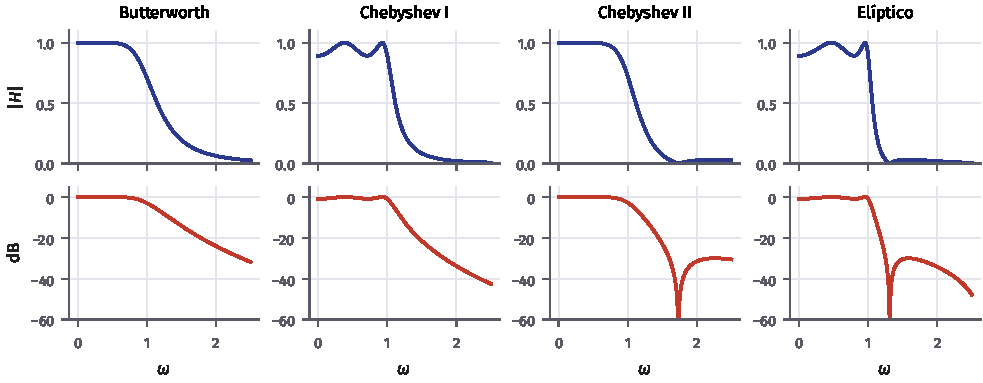
\includegraphics[height=0.42\textheight]{tipos_continuos}\end{center}
  \footnotesize
  \renewcommand{\arraystretch}{1.1}
  \begin{center}
    \begin{tabular}{@{}lllll@{}}
      \toprule
      & Banda de paso & Banda de supresión & Polos / ceros & Fase\\\midrule
      Butterworth & plana & monótona & circunferencia / — & la más lineal\\
      Chebyshev I & rizado & monótona & elipse / — & \\
      Chebyshev II & plana & rizado & — / eje $j\omega$ & \\
      Elíptico & rizado & rizado & — / eje $j\omega$ & la menos lineal\\\bottomrule
    \end{tabular}
  \end{center}
\end{frame}

\begin{frame}{Polos y ceros de cada familia}
  \begin{center}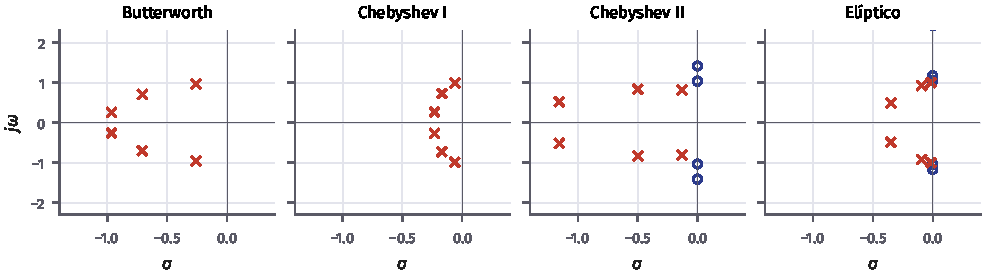
\includegraphics[width=\linewidth]{polos_tipos}\end{center}
  \begin{itemize}\small
    \item Orden 6. Los polos de Chebyshev I están sobre una elipse, más cerca del eje $j\omega$: realzan la banda de paso y producen el rizado.
    \item Los ceros de Chebyshev II y del elíptico, sobre el eje $j\omega$, son los mínimos de la banda de supresión.
  \end{itemize}
  \herramienta{T4-polos-ceros-s}
\end{frame}

\begin{frame}{Ejemplo: las cuatro familias con la misma plantilla}
  \begin{columns}[c]
    \begin{column}{0.56\textwidth}
      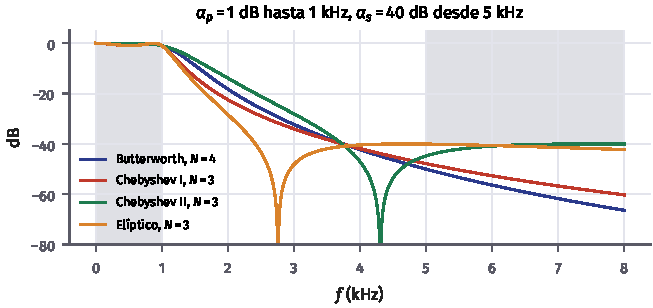
\includegraphics[width=\linewidth]{ejemplo_continuo}
    \end{column}
    \begin{column}{0.42\textwidth}
      \small
      \begin{itemize}
        \item Butterworth necesita $N=4$; los otros tres, $N=3$.
        \item Con $N=3$, el elíptico es el que más margen deja en la banda de supresión.
        \item Chebyshev II es plano en la banda de paso y cumple justo la de supresión.
      \end{itemize}
    \end{column}
  \end{columns}
\end{frame}

\begin{frame}{En código: orden de cada familia}
  \codigo{orden_continuos}
  \nota{Cuidado con el orden de los argumentos: \texttt{cheby1(N,Rp,Wp)}, \texttt{cheby2(N,Rs,Ws)}, \texttt{ellip(N,Rp,Rs,Wp)}, igual en Matlab y en \texttt{scipy.signal}.}
\end{frame}

% =====================================================================
\section{Transformaciones de frecuencia}

\begin{frame}{Del prototipo paso bajo a los demás tipos}
  Se diseña un paso bajo $H_{\text{LP}}(s)$ con $\omega_p=1$ y se sustituye $s$ por una función de $\hat s$:
  \footnotesize
  \renewcommand{\arraystretch}{1.6}
  \begin{center}
    \begin{tabular}{@{}llll@{}}
      \toprule
      Destino & Sustitución & Frecuencias & Datos\\\midrule
      Paso bajo & $s=\hat s/\hat\omega_p$ & $\omega=\hat\omega/\hat\omega_p$ & $\hat\omega_p$\\
      Paso alto & $s=\hat\omega_p/\hat s$ & $\omega=-\hat\omega_p/\hat\omega$ & $\hat\omega_p$\\
      Paso banda & $s=\dfrac{\hat s^2+\hat\omega_0^2}{B\,\hat s}$ & $\omega=\dfrac{\hat\omega^2-\hat\omega_0^2}{B\,\hat\omega}$ & $\hat\omega_0^2=\hat\omega_{p1}\hat\omega_{p2}$, $B=\hat\omega_{p2}-\hat\omega_{p1}$\\
      Supresor & $s=\dfrac{B\,\hat s}{\hat s^2+\hat\omega_0^2}$ & $\omega=\dfrac{B\,\hat\omega}{\hat\omega_0^2-\hat\omega^2}$ & $\hat\omega_0^2=\hat\omega_{p1}\hat\omega_{p2}$, $B=\hat\omega_{p2}-\hat\omega_{p1}$\\\bottomrule
    \end{tabular}
  \end{center}
  \small
  \begin{enumerate}
    \item Llevar los bordes de supresión al prototipo: $\omega_s=\min\abs{\omega(\hat\omega_{s})}$ sobre los bordes dados.
    \item Diseñar el prototipo con $\omega_p=1$, $\omega_s$, $\alpha_p$, $\alpha_s$.
    \item Sustituir: $H(\hat s)=H_{\text{LP}}(s)\big|_{s=F(\hat s)}$ (\texttt{lp2hp}, \texttt{lp2bp}, \texttt{lp2bs}).
  \end{enumerate}
\end{frame}

\begin{frame}{Transformaciones sobre un mismo prototipo}
  \begin{center}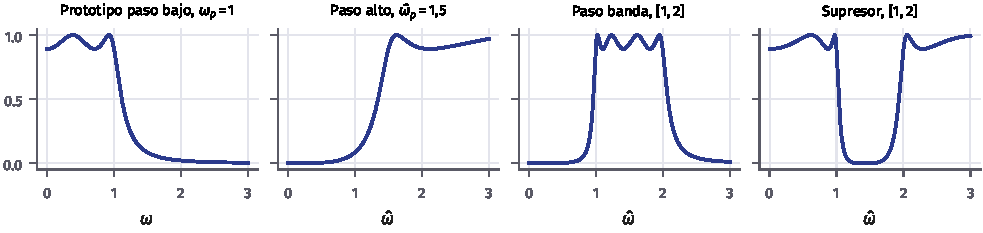
\includegraphics[width=\linewidth]{transformaciones}\end{center}
  \begin{itemize}\small
    \item La transformación conserva los niveles (rizados y atenuaciones) y solo mueve las frecuencias.
    \item El paso banda obtenido es \alert{geométricamente simétrico} respecto a $\hat\omega_0$: $\hat\omega_1\hat\omega_2=\hat\omega_0^2$ para cada par de frecuencias con la misma atenuación. Por eso hay que tomar el borde de supresión más exigente.
    \item El orden se duplica en paso banda y supresor: un prototipo de orden $N$ da $2N$ polos.
  \end{itemize}
\end{frame}

\begin{frame}{Ejemplo: paso alto}
  \begin{ejemplo}[Enunciado]
    Butterworth paso alto: banda de paso desde 4\,kHz con rizado de 0,1\,dB, atenuación mínima de 40\,dB por debajo de 1\,kHz.
  \end{ejemplo}
  \begin{itemize}
    \item Prototipo: $\omega_p=1$ y $\omega_s=\hat\omega_p/\hat\omega_s=4$ (el signo de $\omega=-\hat\omega_p/\hat\omega$ no importa: $\abs{H}$ es par).
    \item $N\ge\dfrac{\log_{10}(9999/0{,}0233)}{2\log_{10}4}=4{,}68\to N=5$.
    \item Paso alto: $H(\hat s)=H_{\text{LP}}(\hat\omega_p/\hat s)$ con $\hat\omega_p=2\pi\cdot4000$\,rad/s.
    \item O todo de una vez con \texttt{butter(N,wn,'high','s')}.
  \end{itemize}
\end{frame}

\begin{frame}{En código: paso alto}
  \codigo[basicstyle=\ttfamily\fontsize{6.8}{7.8}\selectfont]{paso_alto_continuo}
  \nota{Octave no tiene \texttt{lp2hp}; en Matlab y en \texttt{scipy.signal} las dos vías dan el mismo filtro.}
\end{frame}

\begin{frame}{Ejemplos: paso banda y supresor de banda}
  \small
  \begin{ejemplo}[Paso banda elíptico]
    Paso de 4 a 7\,kHz con 1\,dB; supresión por debajo de 3 y por encima de 8\,kHz con 22\,dB. En kHz ($2\pi$ se simplifica): $\hat\omega_0^2=28$, $B=3$,
    \[
      \omega(3)=\frac{\abs{9-28}}{3\cdot3}=2{,}11,\quad \omega(8)=\frac{64-28}{8\cdot3}=1{,}5\ \Rightarrow\ \omega_s=1{,}5,\ N=3\ \text{(orden 6)}.
    \]
  \end{ejemplo}
  \begin{ejemplo}[Supresor Chebyshev II]
    Paso por debajo de 4 y por encima de 7\,kHz con 2\,dB; supresión de 5 a 6\,kHz con 30\,dB. $\hat\omega_0^2=28$, $B=3$:
    \[
      \omega(5)=\frac{5\cdot3}{28-25}=5,\quad \omega(6)=\frac{6\cdot3}{36-28}=2{,}25\ \Rightarrow\ \omega_s=2{,}25,\ N\ge3{,}02\to4.
    \]
  \end{ejemplo}
  \nota{\texttt{cheb2ord} sobre las especificaciones originales devuelve $N=3$: busca los bordes de paso que minimizan el orden. Ambos diseños cumplen la plantilla.}
\end{frame}

% =====================================================================
\section*{Resumen}
\begin{frame}{Conceptos importantes}
  \begin{columns}[T]
    \begin{column}{0.5\textwidth}
      \begin{itemize}
        \item Se diseña $\abs{H(j\omega)}^2=1/(1+P(\omega^2))$ y se toman los polos estables.
        \item Butterworth: plano, $N\ge\log(1/k_1)/\log(1/k)$.
        \item Chebyshev I/II: rizado en una banda, $N\ge\mathrm{arccosh}(1/k_1)/\mathrm{arccosh}(1/k)$.
        \item Elíptico: rizado en ambas, orden mínimo.
      \end{itemize}
    \end{column}
    \begin{column}{0.5\textwidth}
      \begin{itemize}
        \item Más selectividad $\Rightarrow$ fase menos lineal.
        \item Paso alto, paso banda y supresor: prototipo paso bajo y transformación de frecuencias.
        \item Matlab/\texttt{scipy.signal}: \texttt{buttord}, \texttt{cheb1ord}, \texttt{cheb2ord}, \texttt{ellipord} y \texttt{butter}, \texttt{cheby1}, \texttt{cheby2}, \texttt{ellip} con \texttt{'s'} o \texttt{analog=True}.
      \end{itemize}
    \end{column}
  \end{columns}
  \bigskip
  \gris{Apuntes del Tema 4, sección 2 · Hoja de ejercicios, ejercicios 4–7.}
  \herramienta{T4-filtros-continuos}
\end{frame}

\end{document}
